\documentclass[12pt,a4paper,titlepage]{article}
\usepackage[utf8]{inputenc}
\usepackage[english,russian]{babel}
\usepackage[usenames]{color} %!!
\usepackage{colortbl} %!
\usepackage{amsmath}
\usepackage{amsfonts}
\usepackage{amssymb}
\usepackage{mathrsfs}
\usepackage{indentfirst}
\usepackage[hidelinks]{hyperref}
\usepackage[ddmmyyyy]{datetime}
\usepackage{epigraph}
\usepackage{graphicx}
\graphicspath{{fig/}}
\usepackage[subnum]{cases}
\usepackage[left=3cm,right=2cm,top=2cm,bottom=2cm]{geometry}
\DeclareMathOperator{\Div}{div}
\DeclareMathOperator{\Rot}{rot}
\DeclareMathOperator{\Grad}{grad}
\DeclareMathOperator{\Arsh}{Arsh}
\DeclareMathOperator{\const}{const}
\DeclareMathOperator{\inv}{inv}
\newcommand{\parder}[2]{\dfrac{\partial {#1}}{\partial {#2}}}
\newcommand{\vecmult}[2]{\left[ \vec{{#1}} \times \vec{{#2}}   \right]}
\newcommand{\abs}[1]{\left| #1  \right|}
\renewcommand{\vec}[1]{\mathbf{#1}}
\renewcommand{\Re}{\operatorname{Re}}
\renewcommand{\Im}{\operatorname{Im}}

\usepackage{bbold}
\usepackage{mathtools}
\DeclarePairedDelimiter\bra{\langle}{\rvert}
\DeclarePairedDelimiter\ket{\lvert}{\rangle}
\DeclarePairedDelimiterX\braket[2]{\langle}{\rangle}{#1 \delimsize\vert #2}

\date{ }
\author{Petrov M. I.}
\title{\textbf{Quantum Optics} \\ lecture course}


\begin{document}

	\maketitle
	\newpage
	\renewcommand\contentsname{Contents} 
	\tableofcontents

	\section{Secondary quantization}
	
	\subsection{Introduction}
	
	Second quantization starts with an expansion of a scalar or vector field (or wave functions) in a basis consisting of a complete set of functions. These expansion functions depend on the coordinates of a single particle. The expansion coefficients have been promoted from ordinary numbers to operators, creation and annihilation operators. A creation operator creates a particle in the corresponding basis function and an annihilation operator annihilates a particle in this function.
	
	
	\subsection{System for $\vec{A}$}
	
	Let us write Maxwell equations in vacuum without any charge in the system (in CGS units):
	\begin{numcases}{}
		\Rot \vec{E} = - \frac{1}{c} \parder{\vec{H}}{t},
		\label{eq:M1} \\
		\Rot \vec{H} = \frac{1}{c} \parder{\vec{E}}{t},
		\label{eq:M2} \\
		\Div \vec{E} = 0,
		\label{eq:M3} \\
		\Div \vec{H} = 0.
		\label{eq:M4}
	\end{numcases}
	It's more convenient to work with potentials but not the fields itself. If we know $\vec{A}$ и $\varphi$, we know the field
	\begin{eqnarray}
		\vec{E} &=& - \frac{1}{c} \parder{\vec{A}}{t} - \nabla \varphi, \label{eq:E_field}\\
		\vec{H} &=& \Rot \vec{A}.
	\end{eqnarray}
	It's easy to construct two (generally speaking infinitely many) different potential which can lead to the same EM fields. So we can put one arbitrary condition for $\vec{A}$ and $\varphi$. Let us use Lorentz gauge:
	\begin{equation}
		\Div \vec{A} = 0.
		\label{eq:Lorentz}
	\end{equation}
	
	Let us obtain an equation for $\vec{A}$. Substitution of field to the \eqref{eq:M2} gives us
	\begin{equation}
		\Rot \Rot \vec{A} = - \frac{1}{c^2} \parder{^2 \vec{A}}{t^2} - \frac{1}{c} \nabla \parder{\varphi}{t}
	\end{equation}
	and since
	\begin{equation}
		\Rot \Rot \vec{A} = \underbrace{\Grad \Div \vec{A}}_{\hookrightarrow = 0} - \Div \Grad \vec{A} = - \Delta \vec{A}
	\end{equation}
	then
	\begin{equation}
		\Delta \vec{A} - \frac{1}{c^2} \parder{^2 \vec{A}}{t^2} = \frac{1}{c} \nabla \parder{\varphi}{t}.
		\label{eq:temp1}
	\end{equation}
	If we do $\nabla\cdot$\eqref{eq:E_field} then we get
	\begin{equation}
		\underbrace{\Div \vec{E}}_{\hookrightarrow=0} = - \underbrace{\frac{1}{c} \parder{}{t} \Div \vec{A}}_{\hookrightarrow=0} - \Delta \varphi \quad \to \quad \Delta \varphi = 0 \quad \to \quad \nabla \varphi = 0.
	\end{equation}
	So we have system for $\vec{A}$:
	\begin{equation}
		\begin{cases}
			\Delta \vec{A} - \dfrac{1}{c^2} \parder{^2 \vec{A}}{t^2} = 0, \\ \\
			\Div \vec{A} = 0.
		\end{cases}
		\label{eq:forA}
	\end{equation}
	\textit{Remark:} in deriving this system we put $\rho = 0$ and $\vec{j} = 0$.
	
	\subsection{Formulation of the problem}
	
	Let us consider a cube with length of the edge $L$ (fig \ref{fig:cube}). Boundary conditions \textcolor{red}{should be zero or periodic} with the period $L$. System is considered to be conservative. The main idea is to solve system \eqref{eq:forA} and then just find the limit $L \to \infty$.
	
	\begin{figure}
		\centering
		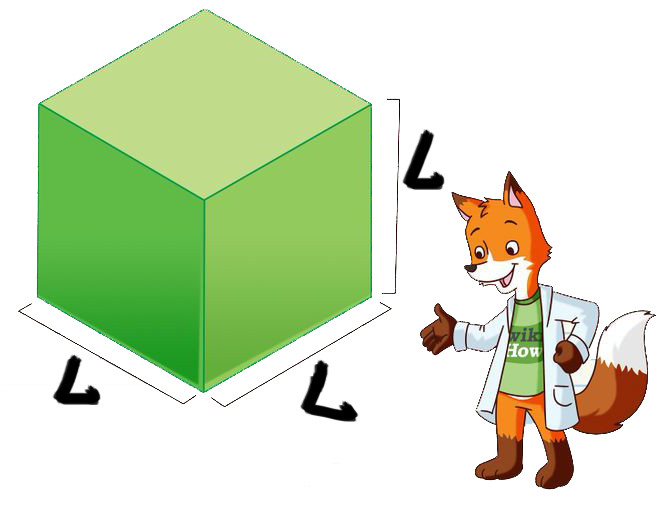
\includegraphics[width=0.5\linewidth]{fig/L1/cube}
		\caption{Formulation of the problem}
		\label{fig:cube}
	\end{figure}

	Solution of \eqref{eq:forA} may be written as the sum of all eigen solutions (each of it is a plane wave) in respect that boundary conditions are periodic:
	\begin{equation}
		\vec{A}(\vec{r},t) = \sum_{\vec{k}} \vec{A}_{\vec{k}}(t) e^{i \vec{k} \vec{r}}, \qquad k_{\alpha} = \frac{2 \pi n_{\alpha}}{L}, \quad \alpha = x,y,z.
	\end{equation}
	%Where $\vec{n}$ --- a unit vector. 
\textcolor{red}{Where $n_{\alpha}$ --- is an integer number.}
As waves are plane then we should write
	\begin{equation}
		\vec{A}_{\vec{k}}(t) = \vec{c}_{\vec{k}} e^{-i \omega_{\vec{k}}t} + \vec{c}_{-\vec{k}}^* e^{i \omega_{\vec{k}}t},
	\end{equation}
	where $\omega_{\vec{k}} = c k = c\sqrt{k_x^2 + k_y^2 + k_z^2}$. 
Let us make a remark: $\vec{A}_{\vec{k}} \in \mathbb{R}$, \textcolor{red}{so
\begin{equation}\label{kminsk}
		\vec{A}_{\vec{k}}(t)=\vec{A}_{\vec{k}}^*(t) = \vec{c}_{-\vec{k}} e^{-i \omega_{\vec{k}}t}+ \vec{c}_{\vec{k}}^* e^{i \omega_{\vec{k}}t}=\vec{A}_{\vec{-k}}(t),
	\end{equation} }.
	The Lorentz gauge leads to the fact that \textit{waves are transverse}:
	\begin{equation}
		\Div \vec{A} = 0 \quad \to \quad \sum \vec{k} \vec{A}_{\vec{k}} e^{i \vec{k} \vec{r}} = 0 \quad \Longleftrightarrow \quad \boxed{\vec{A}_{\vec{k}}(t) \cdot \vec{k} = 0.}
	\end{equation} 
	
	Consider a wave with wave vector $\vec{k}$. According to Maxwell equations, there are two independent polarizations, so we introduce two transverse polarization vectors $\vec{e}_{\vec{k}1}; \vec{e}_{\vec{k}2}$. Three vectors $(\vec{e}_{\vec{k}1}; \vec{e}_{\vec{k}2}; \vec{k}/k)$ form a right-handed orthonormal basis which implies:
	\begin{equation}
		\begin{matrix}
			\vec{k} \cdot \vec{e}_{\vec{k}s} = 0, && \vecmult{\vec{e}_{\vec{k}1}}{\vec{e}_{\vec{k}2}} = \vec{k}/k, \\ \\
			\vec{e}_{\vec{k}s} \cdot \vec{e}_{\vec{k}s'} = \delta_{ss'}, && \vec{c}_{\vec{k}} = \sum_s c_{\vec{k}s} \vec{e}_{\vec{k}s}.
		\end{matrix}
	\end{equation}
	After that we can rewrite decomposition of $\vec{A}$ as
	\begin{multline}
		\vec{A} = \sum_{\vec{k},s} \tilde{A}_{\vec{k}} \left( c_{\vec{k}s} \vec{e}_{\vec{k}s} e^{-i \omega_{\vec{k}} t} + c^*_{-\vec{k}s} \vec{e}^*_{-\vec{k}s}  e^{i \omega_{\vec{k}} t} \right) \cdot e^{i \vec{k} \vec{r}} = \\
		= \left/ \text{inverse 2nd sum \textcolor{red}{using \eqref{kminsk}}: } (-k) \to k \right/ =\sum_{\vec{k},s} \tilde{A}_{\vec{k}} \left( u_{\vec{k}s}(t) \vec{e}_{\vec{k}s} e^{i \vec{k} \vec{r}} + u^*_{\vec{k}s}(t) \vec{e}^*_{\vec{k}s}  e^{-i \vec{k} \vec{r}} \right),
	\end{multline}
	where $u_{\vec{k}s}(t) = c_{\vec{k}s} e^{-i \omega_{\vec{k}} t}$. Now we can write fields
	\begin{equation}
		\vec{E} = -\frac{1}{c} \parder{\vec{A}}{t} = \frac{i}{c} \sum_{\vec{k},s} \tilde{A}_{\vec{k}} \omega_{\vec{k}} \left( u_{\vec{k}s}(t) \vec{e}_{\vec{k}s} e^{i \vec{k} \vec{r}} - u^*_{\vec{k}s}(t) \vec{e}^*_{\vec{k}s}  e^{-i \vec{k} \vec{r}} \right),
	\end{equation}
	\begin{equation}
		\vec{H} = \Rot \vec{A} = i \sum_{\vec{k},s} \tilde{A}_{\vec{k}} \left( u_{\vec{k}s} \left[ \vec{k} \times \vec{e}_{\vec{k}s} \right] e^{i \vec{k} \vec{r}} - u^*_{\vec{k}s} \left[ \vec{k} \times \vec{e}^*_{\vec{k}s} \right] e^{-i \vec{k} \vec{r}} \right).
	\end{equation}
	
	The energy of EM field
	\begin{equation}
		\mathscr{H} = \frac{1}{8 \pi} \int \left(\vec{H}^2 + \vec{E}^2 \right) dV.
	\end{equation} 
	\textit{Remark:} there is no averaging over time!
	
	To make next calculations easier, let us notice that
	\begin{eqnarray}
		\int \limits_{L^3} e^{i (\vec{k} - \vec{k}')\vec{r}} dV = L^3 \delta_{\vec{k}\vec{k}'}.
	\end{eqnarray}
	This feature vanish the $\sum_{\vec{k}}$. Besides, it's convenient to notice that
	\begin{equation}
		\vec{e}_{\vec{k}s}^* \cdot \vec{e}_{\vec{k}s'} = \delta_{ss'} \qquad \to \qquad
		\left[ \vec{k} \times \vec{e}_{\vec{k}s}^* \right] \cdot \left[ \vec{k} \times \vec{e}_{\vec{k}s'} \right] = k^2 \delta_{ss'}.
	\end{equation}
	Then we get
	\begin{equation}
		\mathscr{H} = \frac{L^3}{8 \pi}\textcolor{red}{2} \sum_{\vec{k},s} \tilde{A}_{\vec{k}}^2 \Bigg( \underbrace{\frac{\omega_{\vec{k}}^2}{c^2} \left| u_{\vec{k}s} \right|^2}_{\hookrightarrow E^2} + \underbrace{k^2 \left| u_{\vec{k}s} \right|^2}_{\hookrightarrow H^2}  \Bigg), \qquad k^2 = \frac{\omega_{\vec{k}}^2}{c^2} \text{\ \ (for each mode!)}
	\end{equation}
	\begin{equation}
		\mathscr{H} = \frac{L^3}{\textcolor{red}{2} \pi} \sum_{\vec{k},s} \tilde{A}_{\vec{k}}^2 k^2 \left| u_{\vec{k}s} \right|^2.
	\end{equation}
	Segregation if real and imaginary part of mode can be done by introducing new variables
	\begin{eqnarray}
		q_{\vec{k}s}(t) &=& u_{\vec{k}s}(t) + u^*_{\vec{k}s}(t) , \\
		p_{\vec{k}s}(t) &=& -i \omega_{\vec{k}}  \left( u_{\vec{k}s}(t) - u^*_{\vec{k}s}(t) \right).
	\end{eqnarray}
	It's obvious that
	\begin{equation}
		u_{\vec{k}s}(t) = \frac{1}{2} q_{\vec{k}s}(t) - \frac{1}{2 i \omega} p_{\vec{k}s}(t) \quad \to \quad \left| u_{\vec{k}s} \right|^2 = \frac{1}{4 \omega_{\vec{k}}^2} \left( p^2_{\vec{k}s} + \omega^2_{\vec{k}} q_{\vec{k}s}^2 \right).
	\end{equation}
	The Hamiltonian function will be as follows
	\begin{equation}
		\mathscr{H} = \frac{L^3}{\textcolor{red}{4} \pi c} \sum_{\vec{k},s} \frac{\tilde{A}_{\vec{k}}^2}{2} \left( p^2_{\vec{k}s} + \omega^2_{\vec{k}} q_{\vec{k}s}^2 \right).
	\end{equation}
	Let us boldly put $\tilde{A}_{\vec{k}} = \sqrt{\textcolor{red}{4} \pi c^2/L^3}$, then finally
	\begin{equation}
		\mathscr{H} = \sum_{\vec{k},s}  \left( \frac{p^2_{\vec{k}s}}{2}+ \frac{\omega^2_{\vec{k}} q_{\vec{k}s}^2}{2} \right).
	\end{equation}
	
	If we can write full energy of the system like $\mathscr{H} \sim p^2/2 + \omega^2 q^2/2$, then it means this system can be quantize.  So next, we  \textit{quantize fields}. First of all we need to move to operators by doing
	\begin{equation}
		\begin{cases}
		q_{\vec{k}s} \to \hat{q}_{\vec{k}s}, \\
		p_{\vec{k}s} \to \hat{p}_{\vec{k}s}.
		\end{cases}
	\end{equation}
	After that our Hamiltonian function will transform to Mr. Hamiltonian. 
	Besides, coordinate and impulse operator must obey next commutation relations:
	\begin{equation}
		\left[\hat{q}_{\vec{k}s} ; \hat{p}_{\vec{k}'s'} \right] = i \hbar \delta^{(3)}_{\vec{k}\vec{k}'} \delta_{ss'},
		\label{eq:con1}
	\end{equation} 
	\begin{equation}
		\left[\hat{q}_{\vec{k}s} ; \hat{q}_{\vec{k}'s'} \right] = \left[\hat{p}_{\vec{k}s} ; \hat{p}_{\vec{k}'s'} \right] = 0.
		\label{eq:con2}
	\end{equation}
	Moreover, this operators must be Hermitian because $\mathscr{H}$ stands for real energy which we can measure. Therefore
	\begin{equation}
		\hat{q}_{\vec{k}s} = \hat{q}^{\dagger}_{\vec{k}s}, \qquad \hat{p}_{\vec{k}s} = \hat{p}^{\dagger}_{\vec{k}s}.
		\label{eq:con3}
	\end{equation}
	Relations \eqref{eq:con1}, \eqref{eq:con2} and \eqref{eq:con3} impose conditions for $\hat{q}_{\vec{k}s}$ and $\hat{p}_{\vec{k}s}$.
	Hereafter we can introduce ladder operators:
	\begin{eqnarray}
		\hat{a}_{\vec{k}s}(t) &=& \dfrac{1}{\sqrt{2 \hbar \omega}} \left( \omega \hat{q}_{\vec{k}s} + i \hat{p}_{\vec{k}s} \right), \\ \nonumber \\
		\hat{a}^{\dagger}_{\vec{k}s}(t) &=& \dfrac{1}{\sqrt{2 \hbar \omega}} \left( \omega \hat{q}_{\vec{k}s} - i \hat{p}_{\vec{k}s} \right).
	\end{eqnarray}
	This leads to the useful representation of $\hat{q}_{\vec{k}s}$ and $\hat{p}_{\vec{k}s}$:
	\begin{eqnarray}
		\hat{q}_{\vec{k}s}(t) &=& \sqrt{\dfrac{\hbar}{2 \omega}} \left( \hat{a}^{\dagger}_{\vec{k}s} +  \hat{a}_{\vec{k}s} \right), \\ \nonumber \\
		\hat{p}_{\vec{k}s}(t) &=& i \sqrt{\dfrac{\hbar \omega}{2}} \left( \hat{a}^{\dagger}_{\vec{k}s} -  \hat{a}_{\vec{k}s} \right).
	\end{eqnarray}
	
	Commutation relations can be easily derived from consideration $\left[ \hat{q}_{\vec{k}s} ; \hat{p}_{\vec{k}s} \right]$ in the repre-sentation  of ladder operators and using \eqref{eq:con1} and \eqref{eq:con2}. So we get
	\begin{equation}
		\left[ \hat{a}_{\vec{k},s} ; \hat{a}^{\dagger}_{\vec{k}',s'} \right] = \delta^{(3)}_{\vec{k}\vec{k}'} \delta_{ss'}.
	\end{equation}
	
	Easy to show that Hamiltonian can be written as follows
	\begin{equation}
		\hat{\mathscr{H}} = \sum_{\vec{k},s} \hbar \omega_{\vec{k}} \left[ \hat{a}^{\dagger}_{\vec{k},s} \hat{a}_{\vec{k},s} + \frac{1}{2} \right].
	\end{equation}
	
	
	\section{Coherent states}

\begin{otherlanguage}{russian}
	\epigraph{Из всех родов, видов, сортов и пород людей самая гнусная --- теоретики.}{\sout{А. Куприн} \\Д. А. Байко}
\end{otherlanguage}

\subsection{Eigenfunction}

Let us consider singlemode field.
%only one emission mode
We will be looking for those photons' states which allow us to get more classical world outlook. In particular we want $\hat{\vec{E}}$ be measurable. So, at first, we need to find eigenfunction of annihilation operator $\hat{a}$.

The first naive idea that may come to mind is to check Fock states. Let's look closer at matrix elements
\begin{equation}
	\bra{m} \hat{a} \ket{n} =
	\begin{pmatrix}
		0 & \sqrt{1} & 0 &  \cdots  & 0 & \cdots \\
		0 & 0 & \sqrt{2} &  \cdots & 0 & \cdots \\
		\vdots & \vdots & \ddots & \ddots & \vdots  & \cdots \\
		0 & \vdots & \cdots & 0 & \sqrt{n} & \cdots \\
		\vdots & \vdots & \vdots & \vdots & \vdots & \ddots\\
	\end{pmatrix}.
\end{equation}
Now it's clear that $\ket{n}$ is not a eigenfunction because there are no elements on the main diagonal.

The ordinary procedure to find eigenfunction is the following. $\ket{\alpha}$ should satisfy
\begin{equation}
	\hat{a} \ket{\alpha} = \alpha \ket{\alpha}.
\end{equation}
where $\alpha$ --- eigenvalue.
Fock states form full basis, so we can write
\begin{equation}
	\ket{\alpha} = \sum_{n=0}^{\infty} c_n \ket{n},
\end{equation}
then
\begin{equation}
	\hat{a} \ket{\alpha} = \sum_{n=0}^{\infty} c_n \hat{a} \ket{n} = \sum_{n=0}^{\infty} c_n \sqrt{n} \ket{n-1} = \sum_{n=0}^{\infty} \sqrt{n+1} \ket{n} = \alpha \sum_{n=0}^{\infty} c_n \ket{n},
\end{equation}
which gives the recurrent relation
\begin{equation}
	c_{n+1} \sqrt{n+1} = c_n \alpha \qquad \to \qquad c_n = \frac{\alpha^n}{\sqrt{n!}} c_0 \qquad \to \qquad \ket{\alpha} = c_0 \sum_{n=0}^{\infty} \frac{\alpha^n}{\sqrt{n!}} \ket{n}.
\end{equation}
The constant $c_0$ can be found from the normalization condition:
\begin{equation}
	\braket{\alpha}{\alpha} = 1 \quad \to \quad 1 = \left|c_0\right|^2 \sum_{n,m = 0}^{\infty} \frac{\left( \alpha^* \right)^m \alpha^n}{\sqrt{m!n!}} \underbrace{\braket{m}{n}}_{\hookrightarrow  \delta_{mn}} = \left|c_0\right|^2 \sum_{n = 0}^{\infty} \frac{\left|\alpha\right|^2}{n!},
\end{equation}
\begin{equation}
	c_0 = e^{- \left|\alpha\right|^2/2} e^{i \varphi}
\end{equation}
and finally
\begin{equation}
	\boxed{\ket{\alpha} = e^{- \left|\alpha\right|^2/2} e^{i \varphi} \sum_{n = 0}^{\infty} \frac{\alpha^n}{\sqrt{n!}} \ket{n}.}
\end{equation}
\textit{Remark:} usually phase $\varphi$ is neglected.

\begin{testexample}[How many photons are in coherent state?]
	%\textcolor{red}{(UNCOMMENT THIS LATER! (see source))} \\
	By definition
	\begin{equation}
	\overline{n} = \bra{\alpha} \hat{a}^{\dagger} \hat{a} \ket{\alpha}.
	\end{equation}
	And since
	\begin{eqnarray}
	\hat{a} \ket{\alpha} &=& \alpha \ket{\alpha}, \\
	\bra{\alpha} \hat{a}^{\dagger}  &=& \alpha^* \bra{\alpha},
	\end{eqnarray}
	then
	\begin{equation}
	\overline{n} = \left| \alpha \right|^2.
	\end{equation}
\end{testexample}

Another important thing to calculate. Let us find the probability of $n$ photons be in $\ket{\alpha}$ state:
\begin{equation}
	p_n = \left| \braket{n}{\alpha} \right|^2 = e^{- \left|\alpha\right|^2} \frac{\left|\alpha\right|^{2n}}{n!}.
\end{equation}
Here we obtained the Poisson distribution with dispersion $\sigma = \left|\alpha\right|^2$ (fig \ref{fig:2_1}).
\begin{figure}
	\centering
	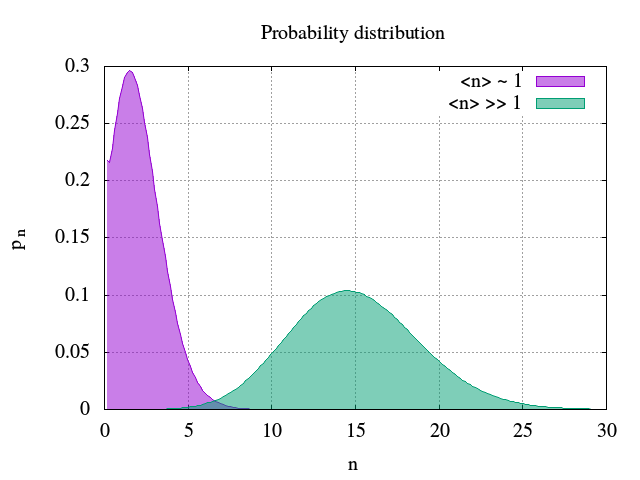
\includegraphics[width=0.7\linewidth]{fig/L2/2_1}
	\caption{Probability distribution for coherent state}
	\label{fig:2_1}
\end{figure}




\begin{hw}[Deadline: 6th of November]
	\addcontentsline{toc}{subsubsection}{Homework}
	\begin{enumerate}
	\item (3 pt) Construct the eigenfunction of the creation operator  $\hat a^{+}|\beta \rangle=\beta|\beta \rangle$.
	
	
	\item (4 pt) Find the eigenfunctions of a coherent state $|\alpha \rangle$ in  the \textbf{position} space (either analytically or numerically).
	
	
	\end{enumerate}
	
	
	{\bf NB:} For solving these problems  you will require the Baker-Campbell-Hausdorff  relations:
	\begin{itemize}
	\item $e^{\hat A+\hat B}=e^{\hat A}e^{\hat B}e^{-\frac{1}{2}[\hat A, \hat B]}$,\ \  if\  $[\hat A,[\hat A,\hat B]]=[\hat B,[\hat B,\hat A]]=[\hat B,[\hat A,\hat B]]=0$
	\item $e^{i\hat A}\hat Be^{-i\hat A} = \hat B + [i\hat A,\hat B] + \dfrac{[i\hat A,[i\hat A,\hat B]]}{2!} + ...$
	\end{itemize}
\end{hw}


\subsection{Orthogonality}

Are coherent states orthogonal or not? Lets find out:
\begin{equation}
	\braket{\alpha'}{\alpha} = e^{- \left|\alpha\right|^2/2} e^{- \left|\alpha'\right|^2/2} \sum \frac{( \accentset{\ast}{\alpha}' )^n \alpha^n}{n!} = e^{-\frac{1}{2} \left|\alpha\right|^2} e^{-\frac{1}{2} \left|\alpha'\right|^2 } e^{\accentset{\ast}{\alpha}' \alpha} \neq 0,
\end{equation}
\begin{equation}
	\left|\braket{\alpha'}{\alpha}\right|^2 = e^{- \left| \alpha - \alpha' \right|^2}.
\end{equation}



\begin{testexample}[If you really want, you can consider coherent states as orthogonal ones!]
	%\textcolor{red}{(UNCOMMENT THIS LATER! (see source))}
	\begin{equation}
	\begin{matrix}
	\ket{\alpha} &=& \ket{3+4i} \\
	\ket{\alpha'} &=& \ket{4+3i} \\
	\end{matrix}
	\quad \to \quad \left|\braket{\alpha'}{\alpha}\right|^2 = e^{-2} \approx 0.1
	\end{equation}
	\begin{equation}
	\begin{matrix}
	\ket{\alpha} &=& \ket{3+4i} \\
	\ket{\alpha'} &=& \ket{-4-3i} \\
	\end{matrix}
	\quad \to \quad \left|\braket{\alpha'}{\alpha}\right|^2  = e^{-98}.
	\end{equation}
	This is a VERY small value!
\end{testexample}

\begin{hw}[Fullness of coherent states.]
Let the reader check the fullness of coherent states. In other words needless to show that
\begin{equation}
	\mathbb{1} = \frac{1}{\pi} \int \limits_{\mathbb{C}} d^2 \alpha \ket{\alpha} \bra{\alpha}.
\end{equation}
\textit{Hint:} for Fock states $\sum_{n=0}^{\infty} \ket{n} \bra{n} = 1$.\\
\textit{Remark:} actually coherent states have the property of overfullness in the sense these states form a basis, but not orthogonal, and one may be expressed with the others.
\end{hw}

Consider the following singlemode field. So this
\begin{equation}
	\hat{\vec{E}} = \sum_{\vec{k},s} \varepsilon_{\vec{k}s} \left( \hat{a}_{\vec{k}s} \vec{e}_{\vec{k}s} e^{i \vec{k} \vec{r} - i \omega_{\vec{k}}t} + \text{ e. c.} \right)
\end{equation}
will be simplified to
\begin{equation}
	\hat{\vec{E}} = \varepsilon \left( \hat{a} \vec{e} e^{i \vec{k} \vec{r} - \omega t} + \text{ e. c.}\right).
\end{equation}
Mean value
\begin{equation}
	\vec{E} = \bra{\alpha} \hat{\vec{E}} \ket{\alpha} = \varepsilon \alpha \vec{e} e^{i \vec{k} \vec{r} - \omega t} + \text{ c. c.} \myeq \vec{E}_+(\vec{r},t) + \vec{E}_-(\vec{r},t).
\end{equation}
The amplitude is defined by $\alpha$:
\begin{equation}
	\vec{E}_+ = E_+ \vec{e} e^{i \vec{k} \vec{r} - \omega t}, \qquad E_+ = \alpha \varepsilon, \qquad \varepsilon = \sqrt{\frac{2 \pi \hbar}{V \omega}}.
\end{equation}
The intensity is proportional to
\begin{equation}
	I_+ \propto \left|E_+\right|^2 = \varepsilon^2 \left|\alpha\right|^2 = \varepsilon^2 \overline{n}.
\end{equation}
From here it is clear that $\varepsilon^2$ stands for the square of electric field amplitude per one photon. Often it is convenient to pick out a phase
\begin{equation}
	E_+ = \varepsilon \left|\alpha\right| e^{i \varphi}.
\end{equation}

Another property of coherent states. Since
\begin{equation}
	\hat{a} \ket{\alpha} = \alpha \ket{\alpha},
\end{equation}
then number of photons in the system does not change! {\textcolor{red}{WAT}}


\begin{hw}[Deadline: 6th of November]
	\addcontentsline{toc}{subsubsection}{Homework}
	
	\begin{enumerate}
	\item (3 pt) Prove the overcompleteness of coherent states:
	$$
	\mathbf{1}=\int_\mathbb{ C} |\alpha\rangle \langle \alpha| \frac{d^{2}\alpha}{\pi}
	$$
	\end{enumerate}


	{\bf NB:} For solving these problems  you will require the Baker-Campbell-Hausdorff  relations:
	\begin{itemize}
	\item $e^{\hat A+\hat B}=e^{\hat A}e^{\hat B}e^{-\frac{1}{2}[\hat A, \hat B]}$,\ \  if\  $[\hat A,[\hat A,\hat B]]=[\hat B,[\hat B,\hat A]]=[\hat B,[\hat A,\hat B]]=0$
	\item $e^{i\hat A}\hat Be^{-i\hat A} = \hat B + [i\hat A,\hat B] + \dfrac{[i\hat A,[i\hat A,\hat B]]}{2!} + ...$
	\end{itemize}

\end{hw}


\subsection{Fluctuations}

Let look at Fock states again. To draw a phase plane we need to remember that
\begin{equation}
	\hat{p} = i \sqrt{\frac{\hbar \omega}{2}} \left( \hat{a}^{\dagger} - \hat{a} \right), \qquad \hat{q} = \sqrt{\frac{\hbar}{2 \omega}}\left( \hat{a}^{\dagger} + \hat{a} \right).
\end{equation}
To find fluctuations let us compute
\begin{equation}
	\overline{p} = \bra{n} \hat{p} \ket{n} = 0, \qquad \overline{q} = \bra{n} \hat{q} \ket{n} = 0
\end{equation}
and
\begin{eqnarray}
	\overline{p^2} = \bra{n} \hat{p}^2 \ket{n} = \frac{\hbar \omega}{2} \left( 2n+1 \right), \\
	\overline{q^2} = \bra{n} \hat{q}^2 \ket{n} = \frac{\hbar}{2 \omega} \left( 2n+1 \right).
\end{eqnarray}
So we have
\begin{equation}
	\Delta p = \sqrt{\overline{p^2} - \overline{p}^2} = \sqrt{\frac{\hbar \omega}{2}} \sqrt{\left( 2n+1 \right)},
\end{equation}
\begin{equation}
	\Delta q = \sqrt{\overline{q^2} - \overline{q}^2} = \sqrt{\frac{\hbar }{2\omega}} \sqrt{\left( 2n+1 \right)}.
\end{equation}
Now we can rewrite the uncertainty principle as following
\begin{equation}
	\Delta p \Delta q = \frac{\hbar}{2} \left(2n+1\right).
\end{equation}

\begin{figure}
	\centering
	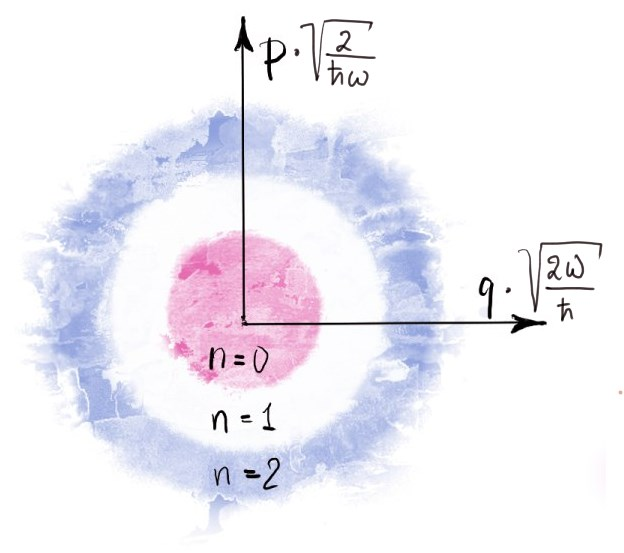
\includegraphics[width=0.4\linewidth]{fig/L2/fluc2}
	\caption{Fluctuations of the Fock states}
	\label{fig:fluc}
\end{figure}

Now let us find the thing for coherent states:
\begin{equation}
	\overline{p} = \bra{\alpha} \hat{p} \ket{\alpha} = i \sqrt{\frac{\hbar \omega}{2}} \left( \alpha^* - \alpha \right) = 2 \sqrt{\frac{\hbar \omega}{2}} \Im \left\{ \alpha \right\},
\end{equation}
\begin{equation}
	\overline{q} = 2 \sqrt{\frac{\hbar }{2\omega}} \Re \left\{\alpha \right\},
\end{equation}
\begin{equation}
	\overline{p^2} = - \frac{\hbar \omega}{2} \bra{\alpha} \hat{a}^{\dagger 2} - \hat{a}^{\dagger} \hat{a} - \hat{a} \hat{a}^{\dagger} + \hat{a}^2  \ket{\alpha} = \frac{\hbar \omega}{2} \left( 4 \Im \left\{ \alpha \right\} + 1\right),
\end{equation}
\begin{equation}
	\overline{q^2} = \frac{\hbar}{2 \omega} \left( 4 \Re \left\{ \alpha \right\} + 1\right).
\end{equation}
Then
\begin{equation}
	\Delta p_{\alpha} = \sqrt{\frac{\hbar \omega}{2} \left[ 4 \Im \left\{ \alpha \right\} + 1 - 4 \Im \left\{ \alpha \right\} \right]^{1/2}} = \frac{\hbar \omega}{2}, \qquad \Delta q_{\alpha} = \frac{\hbar}{2 \omega}.
\end{equation}
The uncertainty relation will be
\begin{equation}
	\boxed{\Delta p_{\alpha} \Delta q_{\alpha} = \frac{\hbar}{2} \quad \slashed{\sim} \quad  \alpha.}
\end{equation}
Here we see that $\Delta p_{\alpha} \Delta q_{\alpha}$ relation does not depend on $\alpha$! In fact we obtained a shifted ground Fock state (fig \ref{fig:shifted_Fock}).

\begin{figure}
	\centering
	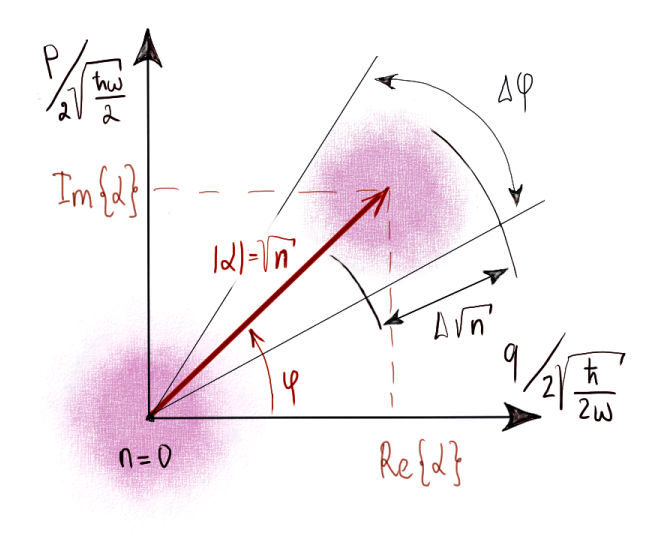
\includegraphics[width=0.6\linewidth]{fig/L2/shifted_Fock1}
	\caption{Shifted Fock states}
	\label{fig:shifted_Fock}
\end{figure}

It conveys the suggestion that a linear operator $\hat{D}(\alpha)$ exist which does this shifting (so-termed \textit{the displacement operator}). In other words
\begin{equation}
	\ket{\alpha} = \hat{D} (\alpha) \ket{0},
\end{equation}
\begin{equation}
	e^{-|\alpha|^2/2} \sum_{n=0}^{\infty} \frac{\alpha^n}{\sqrt{n!}} \ket{n}  = \hat{D} (\alpha) \ket{0},
\end{equation}
and since $\ket{n} = \frac{\left( \hat{a}^{\dagger} \right)^n}{\sqrt{n!}} \ket{0}$, so
\begin{equation}
	D(\alpha) = e^{-|\alpha|^2/2} e^{\alpha \hat{a}^{\dagger}} e^{- \alpha^* \hat{a}}.
\end{equation}
\textit{Remark:} factor $e^{- \alpha^* \hat{a}}$ does not change the result (because $e^{- \alpha^* \hat{a}} \ket{0} = \ket{0}$), but gives some additional properties to the $\hat{D}(\alpha)$:
\begin{enumerate}
	\item Using the Hausdorff relation we can get an alternative from of the displacement operator:
	\begin{equation}
		\hat{D}(\alpha) = e^{\alpha \hat{a}^{\dagger} - \alpha^* \hat{a}}.
	\end{equation}
	\item The displacement operator is a unitary operator. It means that $\hat{D}(\alpha) \hat{D}^{\dagger}(\alpha) = \hat{D}^{\dagger}(\alpha) \hat{D}(\alpha) = \hat{\mathbb{1}}$.
	\item Since $\hat{D}^{\dagger}(\alpha) = \hat{D}(-\alpha)$, the hermitian conjugate of the displacement operator can also be interpreted as a displacement of opposite magnitude.
	\item Following relations hold:
	\begin{eqnarray}
		\hat{D}^{\dagger} (\alpha) \hat{a} \hat{D} (\alpha) &=& \hat{a} + \alpha, \\
		\hat{D} (\alpha) \hat{a} \hat{D}^{\dagger} (\alpha) &=& \hat{a} - \alpha, \\
		\hat{D} (\alpha) \hat{D} (\beta) &=& e^{(\alpha \beta^* - \alpha^* \beta)/2} \hat{D} (\alpha + \beta).
	\end{eqnarray}
\end{enumerate}

In many practical cases a natural question appears: \textit{is it possible to overcome the limit of} $\Delta p_{\alpha} \Delta q_{\alpha} = \frac{\hbar}{2}$ \textit{to get more accurate measurements?}

\begin{hw}[Deadline: 6th of November]
	\addcontentsline{toc}{subsubsection}{Homework}


	\begin{enumerate}
	
	\item (2 pts) Show that the  operator $D(\alpha)=\exp(\alpha\hat{a^\dagger}-\alpha^*\hat{a})$ { displaces} the creation operator by proving the following relations:
	%$$
	%1) D(\alpha)|0\rangle=|\alpha\rangle
	%$$
	$$
	D(\alpha)\hat{a}D(\alpha)^{-1}=\hat{a}-\alpha
	$$
	\item (6 pts) Compute the matrix elements $\langle m| \hat{D}(\alpha)|n\rangle$ of the displacement operator in Fock's basis. Express the result in terms of associated Laguerre polynomials.
	
	\end{enumerate}
	
	
	{\bf NB:} For solving these problems  you will require the Baker-Campbell-Hausdorff  relations:
	\begin{itemize}
	\item $e^{\hat A+\hat B}=e^{\hat A}e^{\hat B}e^{-\frac{1}{2}[\hat A, \hat B]}$,\ \  if\  $[\hat A,[\hat A,\hat B]]=[\hat B,[\hat B,\hat A]]=[\hat B,[\hat A,\hat B]]=0$
	\item $e^{i\hat A}\hat Be^{-i\hat A} = \hat B + [i\hat A,\hat B] + \dfrac{[i\hat A,[i\hat A,\hat B]]}{2!} + ...$
	\end{itemize}
\end{hw}

\subsection{Squeezed states or getting the maximum accuracy!}

Sure, we cannot break the uncertainty principle but we can title the balance of scales for ours good. The main idea is to \textit{squeeze} light state, by geometrical meaning should make an oval from the circle (see fig \ref{fig:sheeeeeeit}).

\begin{figure}[h]
	\begin{minipage}{0.5 \linewidth}
		\center{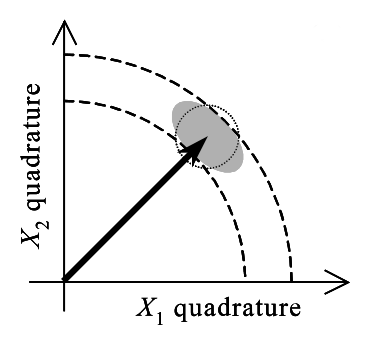
\includegraphics[width=0.7\linewidth]{fig/L2/squeeeeeze_amp} \\ a)}
	\end{minipage}
	\hfill
	\begin{minipage}{0.5 \linewidth}
		\center{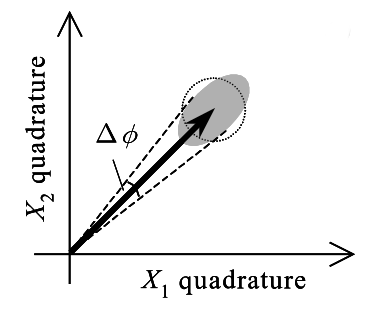
\includegraphics[width=0.7\linewidth]{fig/L2/squeeeeeze_phase} \\ b)}
	\end{minipage}
	\caption{Different light sates on a phase plane: (a) amplitude-squeezed light, (b) phase-squeezed light.}
	\label{fig:sheeeeeeit}
\end{figure}

Let us recall what one property of coherent states
\begin{equation}
	\bra{\alpha} \hat{\vec{E}} \ket{\alpha} = \vec{E} (\vec{r},t).
\end{equation}
From the other hand we have
\begin{equation}
	\bra{n} \hat{\vec{E}} \ket{n} = 0.
\end{equation}
But now if we take into account fluctuations then we get what is shown on fig \ref{fig:noise_MC}. Considering coherent states, lets write a very simplified field time dependence:
\begin{equation}
	E = \varepsilon \left( |\alpha| + \delta \alpha\right) \cos \left[ \omega t + \varphi + \delta \varphi \right],
\end{equation}
where $\delta \alpha$ and $\delta \varphi$ --- fluctuations. For squeezing we will get another picture --- fig \ref{fig:eeeEEeee}.
\begin{figure}
	\centering
	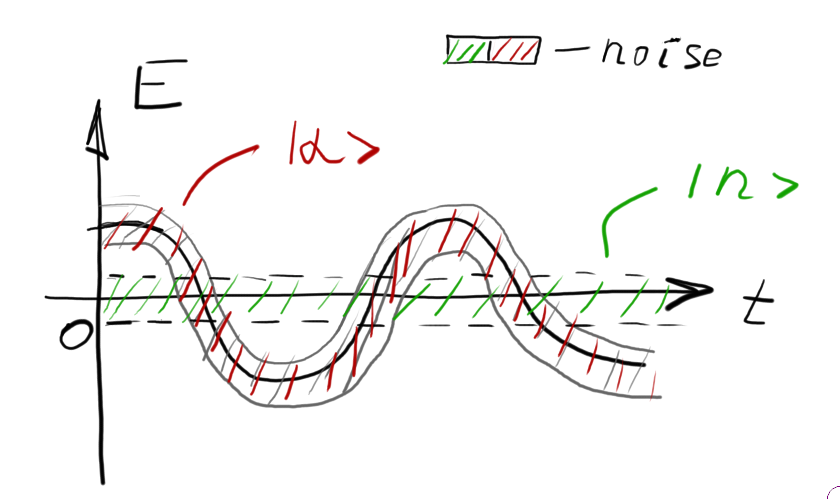
\includegraphics[width=0.65\linewidth]{fig/L2/noise_MC}
	\caption{Field fluctuations for $\ket{\alpha}$ and $\ket{n}$ without squeezing {\textcolor{red}{Here is only ground Fock state shown, next states have greater fluctuations}}}
	\label{fig:noise_MC}
\end{figure}

\begin{figure}
	\centering
	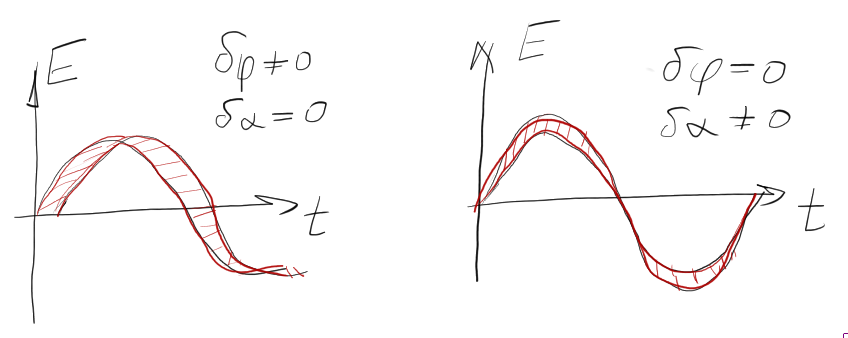
\includegraphics[width=0.7\linewidth]{fig/L2/eeeEEeee}
	\caption{Field fluctuations for squeezed light}
	\label{fig:eeeEEeee}
\end{figure}

To get quantitative and more specific description one can use \textit{the squeeze operator}:
\begin{equation}
	\hat{S} \left( \xi \right) \ket{\alpha} = \ket{\alpha, \xi},
\end{equation}
where $|\xi|$ --- ratio of the main semiaxes of squeezed state, $\arg  \xi $ --- a turning angle.

Here are some helpful properties of the squeeze operator:
\begin{enumerate}
	\item It make be written as following:
	\begin{equation}
		\hat{S} = e^{\xi \hat{a}^{\dagger 2} - \xi^* \hat{a}^2}.
		\label{eq:SS}
	\end{equation}
	\item It is commutative with displacement operator:
	\begin{equation}
		\hat{S} (\xi) \hat{D} (\alpha) \neq  \hat{D} (\alpha) \hat{S} (\xi).
	\end{equation}
\end{enumerate}

Lets draw attention to \eqref{eq:SS}. We can notice that squeeze operator $\hat{S}$ consist of squares of ladder operators ($\sim \hat{a}^{\dagger 2}, \hat{a}^{2}$). It means here we have a generation of second harmonic ($2 \hbar \omega$ instead of $\hbar \omega$). In other words,  from a experimenter's point of view, to get the squeezed state one needs a non-linear optical element with $\chi_2 \neq 0$, so it's polarizability $P = \chi_1 E + \chi_2 E^2$. 



\begin{hw}[Deadline: 6th of November]
	\addcontentsline{toc}{subsubsection}{Homework}

	\begin{enumerate}
		\item (4 pt) {\bfseries Classical squeezing.}\\
		For the problem of a classical harmonic oscillator a general solution can be expressed as $x(t) = c_1 cos\omega_0t + c_2 sin \omega_0t$, where $c_1$ and $c_2$ depend on the  initial conditions. Now consider that you drive this system on a $2\omega_0$ frequency so that $ V(t) = \frac{1}{2}m\omega_0^2x^2\left(1 + \epsilon sin2\omega_0t \right)$ ($\epsilon << 1$). Prove that $c_1(t) = e^{\beta t}$ and $c_2(t) = e^{-\beta t}$ and find $\beta$ using the second Newton's law, the method of  variation of parameters, considering $c_1(t)$ and $c_2(t)$ as slowly varying variables and ignoring fast-oscillating terms.
		
		\item (5 pt) {\bfseries Quantum squeezing.}\\
		Now you know that for squeezing you need to drive your system at $2\omega_0$ frequency. In quantum case it corresponds to the process of parametric down-conversion when you have a strong coherent field (mode $b$) with a frequency $2 \omega_0$ as an input and on the output you have two photons of frequency $\omega_0$ (mode $a$). It can expressed with the following Hamiltonian $\hat H = \hat a^\dagger \hat a^\dagger \hat b + \hat a \hat a \hat b^\dagger$. The corresponding squeezing operator is $\hat S(r) = exp\left[-\frac{r}{2}\left( \hat a^2 - \hat a^{\dagger 2}\right)\right]$, here $r$ describes the strength of squeezing. Compute \\
		$$1) \hat S(r) \hat x \hat S^\dagger (r)$$
		$$2) \hat S(r) \hat p \hat S^\dagger (r)$$
		where $\hat x = \frac{\hat a + \hat a^\dagger}{\sqrt[]{2}}$ and $\hat p = \frac{\hat a - \hat a^\dagger}{\sqrt[]{2}}$.
	\end{enumerate}

	{\bf NB:} For solving these problems  you will require the Baker-Campbell-Hausdorff  relations:
	\begin{itemize}
		\item $e^{\hat A+\hat B}=e^{\hat A}e^{\hat B}e^{-\frac{1}{2}[\hat A, \hat B]}$,\ \  if\  $[\hat A,[\hat A,\hat B]]=[\hat B,[\hat B,\hat A]]=[\hat B,[\hat A,\hat B]]=0$
		\item $e^{i\hat A}\hat Be^{-i\hat A} = \hat B + [i\hat A,\hat B] + \dfrac{[i\hat A,[i\hat A,\hat B]]}{2!} + ...$
	\end{itemize}
\end{hw}

	
\end{document} 